\documentclass[letterpaper,12pt]{article}

\usepackage[spanish, es-tabla]{babel}
\usepackage{graphicx}

\author{Beatriz Garcia L}
\title{Sistema de gestión de una Biblioteca Universitaria}
\date{\today}

\begin{document}
\maketitle

\tableofcontents

\section{Contexto}
Una biblioteca universitaria necesita digitalizar su operación. Actualmente lleva el control en papel y requiere un sistema computacional que gestione su acervo, los prestamos y los usuarios.

\section{Descripción del dominio}

La biblioteca cuenta con \textbf{libro}, de los cuales puede tener varios ejemplares físicos para cada título. Cada libro tienen un título, año de publicación, ISBN y pertenece a una o mas categorías (Ciencias, Humanidades, Ingeniería, etc.). Además, cada libro fue escrito por uno o más autores.

Los usuarios pueden ser estudiantes o profesores. De cada uno se guarda el nombre, correo , número de cuenta y tipo. Un usuario puede tener activos varios préstamos simultáneos (máximo 3), pero un ejemplar solo puede estar prestado a un usuario a la vez.

Cada préstamo registra la fecha de salida, la fecha de devolución esperada y la fecha real de devolución (en el caso de que ya se haya devuelto el ejemplar). Si un préstamo se devuelve más tarde, se registra una multa con el monto y si fue pagada o no.

\section{Modelo entidad-relación \textit{DER}}


\begin{figure}[!h]
    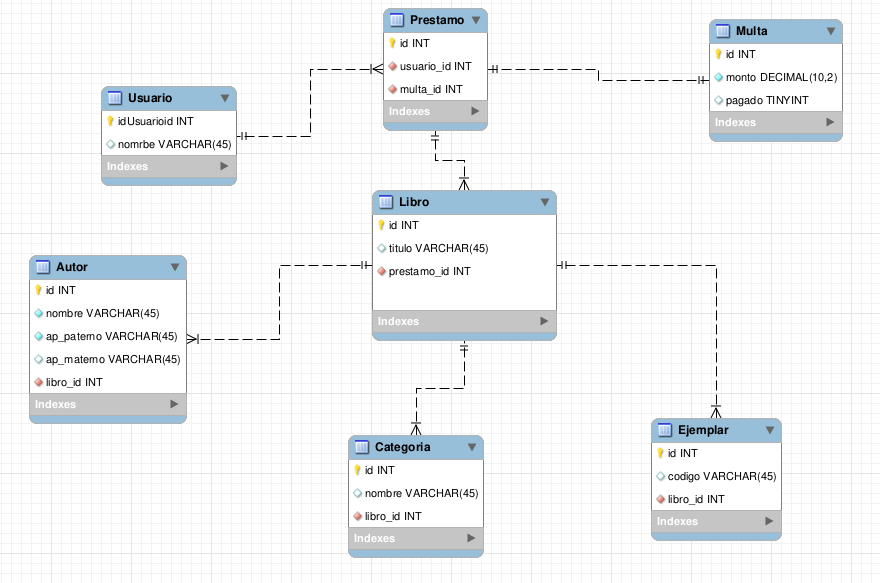
\includegraphics[scale=0.4]{images/der.png}
    \caption{Modelo entidad relación para la biblioteca Universitaria}
    \label{fig_der}
\end{figure}

\begin{table}
    \begin{tabular}{| c | c |}
        \hline
        ¿Qué identificar? & Pista \\
        \hline
        Entidades & ¿Qué cosa del dominio tiene datos propios? \\
        Atributos clave & ¿Qué identifica unívocamente cada entidad?\\
        Relaciones & ¿Cómo se vinculan entre sí?\\
        Entidades débiles & ¿Hay alguna que exista sin otra?\\      
        \hline
    \end{tabular}
    \caption{Identificación de entidades y relaciones}
    \label{tbl_er}
\end{table}

\section{Implementación del modelo en MySQL}

De acuerdo con nuestro DER, figura \ref{fig_der}, creamos los scripts para la implementación.

\end{document}